%& C:\Users\NAGARAJ\AppData\Roaming\TikzEdt\TikzEdt\023~1.0\TEMP_H~1
\begin{document}
\begin{tikzpicture}

\draw [ thick, fill=cyan] (-10.3,-10.25) rectangle (-9.3,-11.25);
\draw [thick] (-10.3,-11.25) rectangle (-9.3,-12.25);
\draw [ thick, fill=cyan] (-10.3,-12.25) rectangle (-9.3,-13.25);
\draw [thick] (-10.3,-13.25) rectangle (-9.3,-14.25);
\draw [thick] (-10.3,-14.25) rectangle (-9.3,-15.25);
\draw [thick] (-10.3,-15.25) rectangle (-9.3,-16.25);
\draw [ thick, fill=cyan] (-10.3,-16.25) rectangle (-9.3,-17.25);
\draw [thick] (-10.3,-17.25) rectangle (-9.3,-18.25);


\node (v2) at (-9.8,-10.75) {\Large  \color{red}$1$};
\node (v4) at (-9.8,-11.75) {\Large \color{red}$2$};
\node (v11) at (-9.8,-12.75) {\Large  \color{red}$3$};
\node (v5) at (-9.8,-13.75) {\Large  \color{red}$4$};
\node (v12) at (-9.8,-14.75) {\Large  \color{red}$5$};
\node (v7) at (-9.8,-15.75) {\Large  \color{red}$6$};
\node (v9) at (-9.75,-16.75) {\Large \color{red}$7$};
\node (v10) at (-9.8,-17.75) {\Large  \color{red}$8$};



% Test1
\draw [] (-4.1,-12.65) rectangle (-3.1,-11.65);
\draw [] (-3.1,-12.65) rectangle (-2.1,-11.65);
\draw [] (-2.1,-12.65) rectangle (-1.1,-11.65) node (v1) {};
\draw [] (v1) rectangle (-0.1,-12.65);
\draw [] (-0.1,-11.65) rectangle (0.9,-12.65);

\node at (-4.15,-13.65) {\Large $\bf{a_1}$ = };
\node at (-3.6,-12.05) {\Large \color{red}2};
\node at (-2.6,-12.05) {\Large \color{red} 4};
\node at (-1.6,-12.05) {\Large \color{red} 5};
\node at (-0.6,-12.05) {\Large \color{red} 6};
\node at (0.4,-12.05) {\Large \color{red} 8};




\node at (-2.75,-13.65) {\Large 0};
\node at (-2.15,-13.65) {\Large 1};
\node at (-1.55,-13.65) {\Large 0};
\node at (-0.95,-13.65) {\Large 1};
\node at (-0.35,-13.65) {\Large 1};
\node at (0.25,-13.65) {\Large 1};
\node at (0.75,-13.65) {\Large 0};
\node at (1.25,-13.65) {\Large 1};
\node at (-3.25,-13.65) {\Large [};
\node at (1.65,-13.65) {\Large ]};






%Test-2
\draw [ fill=cyan] (-4,-8) rectangle (-3,-9);
\draw [] (-3,-8) rectangle (-2,-9);
\draw [](-2,-8) rectangle (-1,-9);

\node at (-4.25,-9.9) {\Large $\bf{a_2}$ = };

\node at (-3.5,-8.4) {\Large \color{red}1};
\node at (-2.5,-8.4) {\Large \color{red} 2};
\node at (-1.5,-8.4) {\Large \color{red} 4};


\node at (-2.85,-9.9) {\Large 1};
\node at (-2.25,-9.9) {\Large 1};
\node at (-1.65,-9.9) {\Large 0};
\node at (-1.05,-9.9) {\Large 1};
\node at (-0.45,-9.9) {\Large 0};
\node at (0.15,-9.9) {\Large 0};
\node at (0.65,-9.9) {\Large 0};
\node at (1.15,-9.9) {\Large 0};
\node at (-3.35,-9.9) {\Large [};
\node at (1.55,-9.9) {\Large ]};

%Test-3
\draw [ ] (-4,-15.15) rectangle (-3,-16.15);
\draw [fill=cyan] (-3,-15.15) rectangle (-2,-16.15);
\draw [] (-2,-15.15) rectangle (-1,-16.15);

\node at (-4.25,-17.15) {\Large $\bf{a_3}$ = };
\node at (-3.5,-15.65) {\Large \color{red}2};
\node at (-2.5,-15.65) {\Large \color{red} 3};
\node at (-1.5,-15.65) {\Large \color{red} 5};

\node at (-3.4,-17.15) {\Large 0};
\node at (-2.8,-17.15) {\Large 0};
\node at (-2.2,-17.15) {\Large 1};
\node at (-1.6,-17.15) {\Large 1};
\node at (-1,-17.15) {\Large 0};
\node at (-0.4,-17.15) {\Large 1};
\node at (0.1,-17.15) {\Large 0};
\node at (0.6,-17.15) {\Large 0};
\node at (-3.65,-17.15) {\Large [};
\node at (1,-17.15) {\Large ]};

%Test-4

\draw [ ] (-4,-18.9) rectangle (-3,-19.9);
\draw [fill=cyan] (-3,-18.9) rectangle (-2,-19.9);
\draw [] (-2,-18.9) rectangle (-1,-19.9);

\node at (-4.3,-20.9) {\Large $\bf{a_4}$ = };
\node at (-3.5,-19.4) {\Large \color{red}6};
\node at (-2.5,-19.4) {\Large \color{red} 7};
\node at (-1.5,-19.4) {\Large \color{red} 8};

\node at (-3.3,-20.9) {\Large 0};
\node at (-2.7,-20.9) {\Large 0};
\node at (-2.1,-20.9) {\Large 0};
\node at (-1.5,-20.9) {\Large 0};
\node at (-0.9,-20.9) {\Large 0};
\node at (-0.3,-20.9) {\Large 1};
\node at (0.2,-20.9) {\Large 1};
\node at (0.7,-20.9) {\Large 1};
\node at (-3.6,-20.9) {\Large [};
\node at (1.1,-20.9) {\Large ]};

\node at (6.2,-4.65) {\Large Test Results  (Observations)};
\node [draw, color=red ] at (6.1,-5.65) {\Large \color{blue} $y_i = \overset{N}{\underset{j=1 }{\vee}} a_{ij}X_j = <a_i , X> $ };


\node at (6,-11.65) {\Large \color{red} Negative};
\node at (6,-12.65) {\Large \color{blue} $y_1 = 0$ };
\node at (6,-7.85) {\Large \color{red} Positive};
\node at (6,-9.05) {\Large \color{blue} $y_1 = 1$};
\node at (6,-15.1) {\Large \color{red}  Positive};
\node at (6,-16.4) {\Large \color{blue} $y_1 = 1$};
\node at (6,-18.9) {\Large \color{red} Positive};
\node at (6,-20.2) {\Large \color{blue} $y_1 = 1$};

\node (v13) at (-4.6,-12.1) {};
\node (v3) at (-4.5,-8.25) {};
\node (v6) at (-4.5,-15.8) {};
\node (v8) at (-4.5,-19.35) {};
\draw  (-4.55,-11.2) rectangle (1.4,-13.1);
\draw  (-4.5,-7.6) rectangle (-0.55,-9.35);
\draw  (-4.5,-14.7) rectangle (-0.5,-16.65);
\draw  (-4.5,-18.45) rectangle (-0.5,-20.35);


\draw [thick,color=blue] (v2) edge (v3);
\draw  [thick,color=blue] (v4) edge (v3);
\draw [thick,color=blue] (v5) edge (v3);



\draw [thick,color=black] (v7) edge (v8);
\draw  [thick,color=black](v9) edge (v8);
\draw  [thick,color=black](v10) edge (v8);

\draw [thick,color=violet] (v4) edge (v6);
\draw [thick,color=violet] (v11) edge (v6);
\draw [thick,color=violet] (v12) edge (v6);

\draw [thick,color=red] (v4) edge (v13);
\draw [thick,color=red] (v5) edge (v13);
\draw [thick,color=red] (v12) edge (v13);
\draw [thick,color=red] (v7) edge (v13);
\draw [thick,color=red] (v10) edge (v13);


\node at (-10,-19.5) {\Large $X$=[1 \ 0 \ 1 \ 0 \ 0 \ 0 \ 1 \ 0]};
\node at (-2.55,-7.3) {\Large \color{blue} Test-1};
\node at (-2.55,-10.95) {\Large \color{blue} Test-2};
\node at (-2.55,-14.5) {\Large \color{blue} Test-3};
\node at (-2.55,-18.2) {\Large \color{blue} Test-4};

\usetikzlibrary{calc}
\pgftransformreset
\node[inner sep=0pt,outer sep=0pt,minimum size=0pt,line width=0pt,text width=0pt,text height=0pt] at (current bounding box) {};
%add border to avoid cropping by pdflibnet
\foreach \border in {0.1}
  \useasboundingbox (current bounding box.south west)+(-\border,-\border) rectangle (current bounding box.north east)+(\border,\border);
\newwrite\metadatafile
\immediate\openout\metadatafile=\jobname_BB.txt
\path
  let
    \p1=(current bounding box.south west),
    \p2=(current bounding box.north east)
  in
  node[inner sep=0pt,outer sep=0pt,minimum size=0pt,line width=0pt,text width=0pt,text height=0pt,draw=white] at (current bounding box) {
\immediate\write\metadatafile{\p1,\p2}
};
\immediate\closeout\metadatafile
\end{tikzpicture}

\end{document}
